\chapter{Discussion}
\label{Chapter:Discussion}

The numerical results allow us to assess how the proposed linearized QAOA protocols compare to the standard formulation and to evaluate the role of the cost function in shaping their performance.

\subsection*{Standard versus linear\_quadratic protocols}

Since both the \texttt{standard} and \texttt{linear\_quadratic} protocols are optimized with respect to the same cost function, $\langle \hat{H}_\mathrm{QP} \rangle$, their performance can be directly compared. The data clearly indicate that the \texttt{linear\_quadratic} protocol reaches relevant solutions with acceptable fidelity at shallower circuit depths. Moreover, when performance is measured against the number of two-qubit gates—a more meaningful indicator of quantum resource requirements—the linear protocol consistently requires fewer resources to achieve comparable or superior fidelities. This indicates that the linearization strategy focuses the optimization on the parts of the problem Hamiltonian that matter most, allowing the algorithm to reach good solutions with less computational effort.

\subsection*{Impact of the cost function}

The choice of cost function proves to be a decisive factor. Between the two linearized protocols, \texttt{linear\_abs} generally outperforms \texttt{linear\_quadratic}, achieving higher fidelities at lower resource counts. This highlights that even within a fixed ansatz structure, selecting a cost function that better reflects the problem's energy landscape can significantly enhance performance. This observation could motivate further investigation into whether alternative ways of defining the cost function might offer performance benefits.

\subsection*{Sudden fidelity jumps in linear protocols}

One of the most distinctive features of the linear protocols is the occurrence of abrupt fidelity jumps as the number of QAOA layers increases. This contrasts with the smoother fidelity evolution observed for the standard protocol, a behavior consistently seen across the problem sizes studied (see Appendix X). To understand this behavior, we analyzed the spectra of the problem Hamiltonians $\hat{H}_\mathrm{LP}$ and $\hat{H}_\mathrm{QP}$, shown in Fig.~\ref{fig:spectrums}.
\begin{figure}[h]
    \centering
    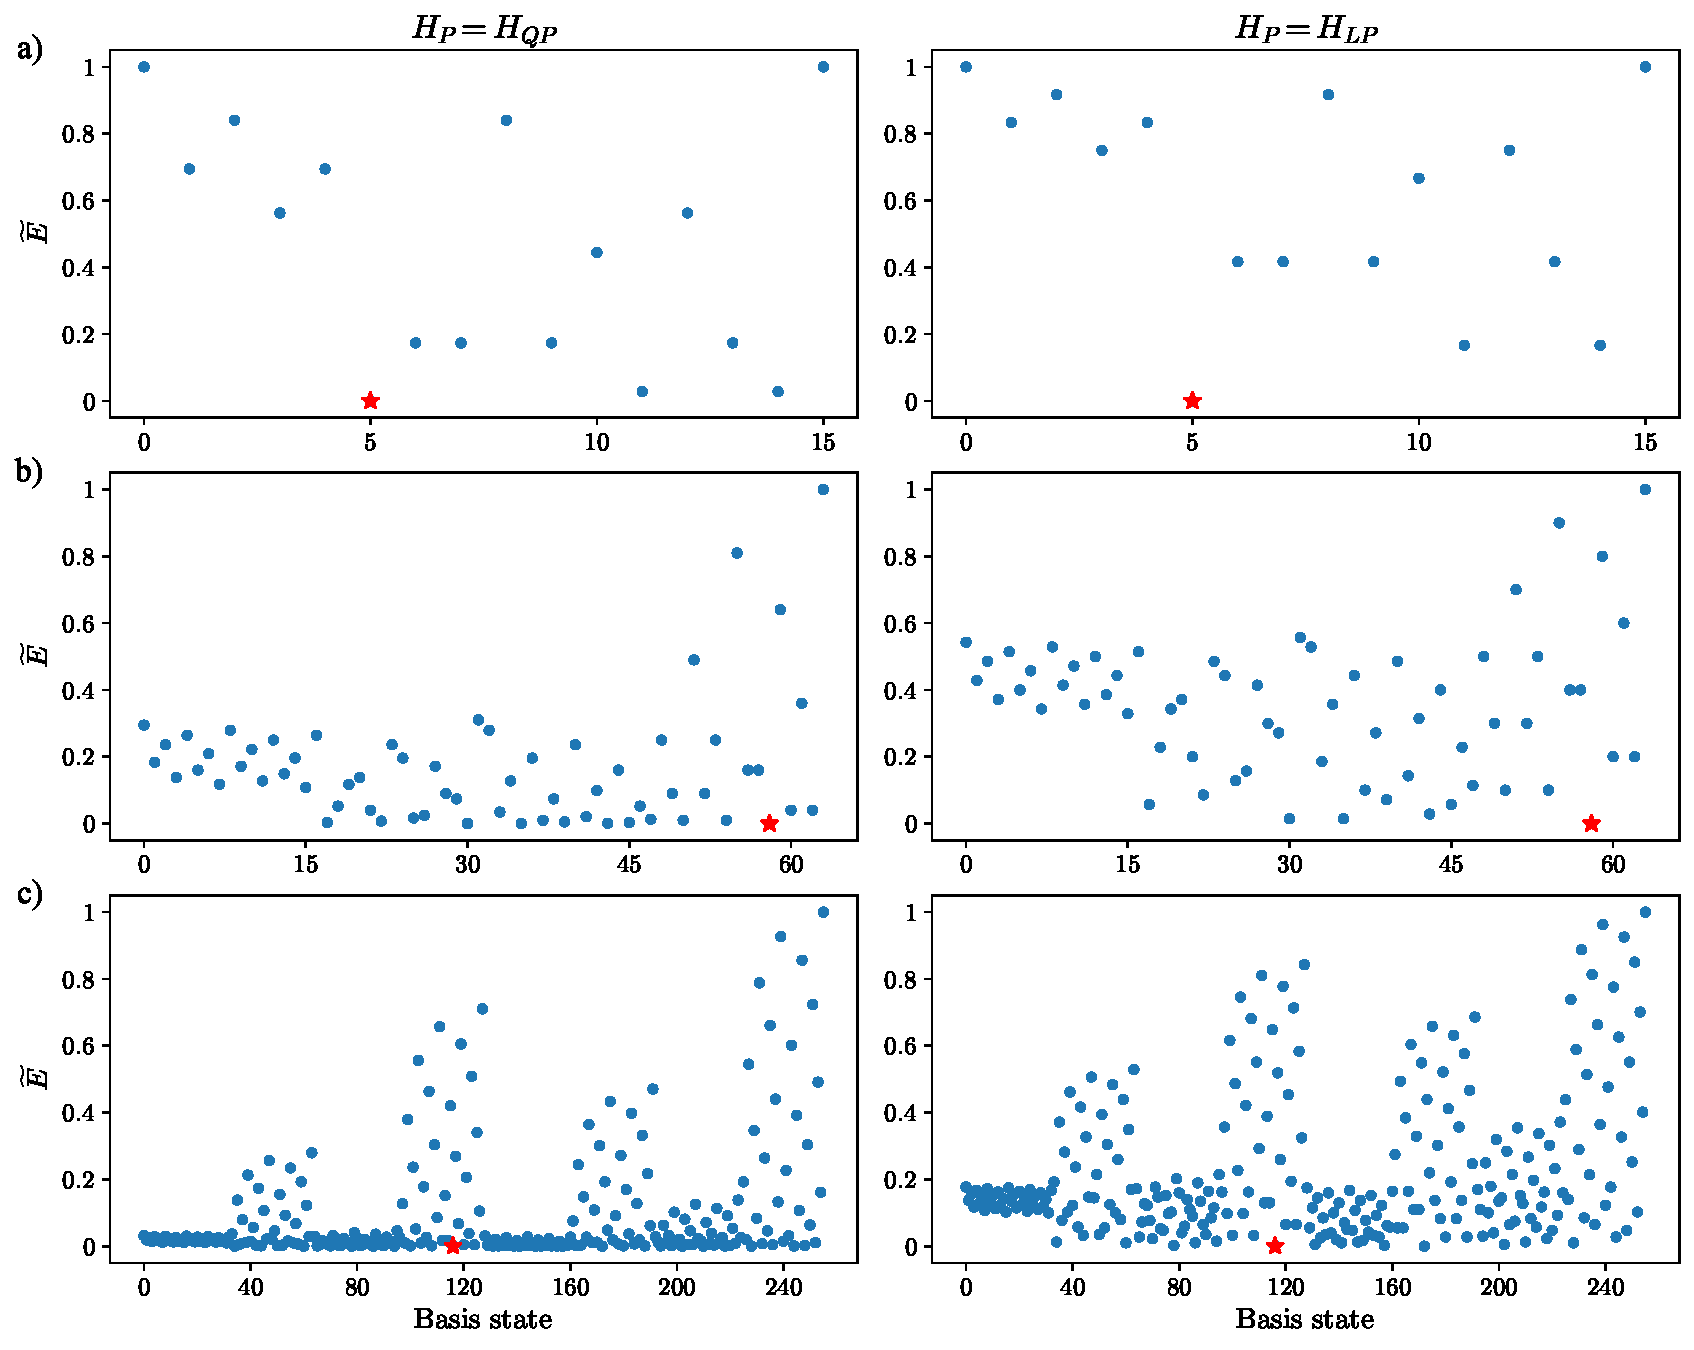
\includegraphics[width=0.96\textwidth]{05-discussion/figs/energy_spectrums.pdf}
    \caption{Energy spectrums for (a) $N=25$, (b) $N=77$, and (c) $N=143$. The horizontal axis shows the decimal encoding of computational basis states, while the vertical axis indicates the normalized eigenenergies. These plots illustrate the broader spectral spread of the linear protocol compared to the quadratic case, which underlies the abrupt fidelity jumps discussed in the text. The eigenstate corresponding to the solution ($\widetilde{E}=0$) is marked as a red star.}
    \label{fig:spectrums}
\end{figure}
We find that the spectrum of $\hat{H}_\mathrm{LP}$ is more widely spread, leading to larger separations between relevant energy levels. Such a structure tends to promote population transfer in discrete steps, which aligns with the observed fidelity jumps. Conversely, the denser spectrum of $\hat{H}_\mathrm{QP}$ supports a more gradual redistribution of amplitude during the variational evolution.

This qualitative picture is further supported by the numerical results summarized in Table~\ref{table:rms}. To quantify the spread of the spectra, we use the root-mean-square (RMS) distance of the eigenvalues with respect to the target energy, which provides a compact measure of how widely distributed the eigenvalues are for each Hamiltonian:
\begin{equation}
    \textrm{RMS} = \sqrt{\dfrac{1}{d} \sum_{i=1}^{d}\widetilde{E}_i^2}\,,
    \label{eq:rms}
\end{equation}
where $\widetilde{E}_i^2$ is the normalized energy of the $i$-th eigenstate.

The results confirm that $\hat{H}_\mathrm{LP}$ consistently exhibits larger RMS distances than $\hat{H}_\mathrm{QP}$ across the problem sizes studied, in agreement with the visual differences in Fig.~\ref{fig:spectrums}. Together, the table and spectra illustrate that the wider separation of eigenvalues in $\hat{H}_\mathrm{LP}$ explains the step-like fidelity behavior observed in the linear protocol.

\begin{table}[h]
    \centering
    \begin{tabular}{@{}lcccccc@{}}
        \toprule
        & \multicolumn{6}{c}{$n$} \\
        \cmidrule(lr){2-7}
        Protocol            & 3     & 4     & 5     & 6     & 7     & 8 \\
        \midrule
        \texttt{standard}   & 0.59  & 0.58  & 0.26  & 0.24  & 0.20  & 0.21 \\
        \texttt{linear}     & 0.70  & 0.68  & 0.41  & 0.37  & 0.32  & 0.32 \\
        \bottomrule
    \end{tabular}
    \caption{Root-mean-square (RMS) distance of the energy spectrum from the target state, used as a measure of how widely the eigenvalues are distributed for each Hamiltonian and problem size.}
    \label{table:rms}
\end{table}

\section{Future prospects}

While the current study focuses on semiprime integers $N$ of moderate size, extending the analysis to larger numbers is pivotal to properly determine whether our results persist in more challenging regimes of factorization. Such investigations would provide a clearer assessment of the asymptotic potential of linearized QAOA and inform the design of more resource-efficient formulations. From an experimental standpoint, our approach offers the additional advantage of requiring only simple quantum circuits, with operations involving at most two qubits. This reduction in circuit complexity significantly enhances the feasibility of near-term realizations on existing hardwares.
